\documentclass[a4paper]{article}

\usepackage{microtype}
\usepackage[english]{babel}
\usepackage{fancyhdr}
\usepackage[colorlinks=true]{hyperref}
\usepackage{graphicx}
\usepackage{todonotes}

\title{\textsc{EnVe 2014: High Voltage} \\ \textbf{Work Package 2}}
\author{Khanh Phanh}
\date{Late Updated: \today}

\begin{document}
\pagestyle{fancy} \lhead{} \rhead{}
\maketitle
\tableofcontents

\section{Tasks: Drive and Control}
    \begin{enumerate}
        \item CAD schematics of feedback systems controlling the motor, how they
        work and how they are connected

        \item A proposal for the control system including the gear involved.
        How the accelerator will be connected to the motor?

        \item To speak with the REV team and any other team currently or that has
        built an electric car and ask them about HV related problems that they had
        and how they solved them
    \end{enumerate}

\section{Control Systems Introduction}
    A little terminology;
        \footnote{\url{https://web.stanford.edu/~boyd/ee102/ctrl-static.pdf}}
        \begin{itemize}
        \item The system to be controlled is called the \textit{plant}
        \item The \textit{sensor} measures the quantity to be controlled
        \item the \textit{actuator} affects/changes the plant
        \item the \textit{controller} or \textit{control processor} processes the
        sensor signal to drive the actuator
        \item the \textit{control law/algorithm} is the algorithm used by the
        control processor to drive the actuator signal
        \end{itemize}

    \begin{figure}
        \centering
        \includegraphics[width=\linewidth]{./images/2_feedbackSystems}
    \end{figure}

   \subsection{Functions of Motor Control}
    Some function to keep in mind for the design of the motor control system
        \footnote{\url{http://www.ohioelectricmotors.com/a-guide-to-electric-drives-and-dc-motor-control-688}}
    \begin{itemize}
    \item Starting
    \item Stopping
    \item Jogging/Inching
    \item Plugging
    \item Speed Control
    \item Reversing
    \item Braking
    \item Protection
    \end{itemize}

\section{DC Motor Controls}
    Back EM Field Weakening control to achieve higher top speeds\todo{Not sure
    about this; google "field weakning control"}
        \footnote{\url{http://web.eecs.utk.edu/~tolbert/power_electronics/pubs/Chiasson_publications_04.pdf}}

\section{BLDC Motor Control}
    BLDC control schemes are mainly classified in the following two types
    \begin{itemize}
    \item Sensor Based Control
    \item Sensorless Based Conrol
    \end{itemize}

\subsection{BLDC Motor Sensor Control}
    BLDC commutation is performed electronically;
    The key to BLDC commutation is to determine the rotor position relative to
    the stator coils, and
    accordingly energize the phases in which will produce the most torque.
    Theoretically, and most likely practically, maximum torque is produced when
    the rotor is orthogonal to the alignment of the stator magnetic field.
        \footnote{\url{http://edge.rit.edu/content/P10022/public/team_docs/Files_To_Be_Deleted/team_docs/technical_literature/Brushless_DC_Motor_Control_Made_Easy.pdf}}

    Typically, a Hall sensor is used, which detects the position of the rotor
    magnet and gives a signal which is used to give appropriate excitation to
    the stator windings, as per above
        \footnote{\url{http://www.academia.edu/7101951/MICROCONTROLLER_BASED_CONTROL_OF_THREE_PHASE_BLDC_MOTOR}}

    Hall sensors work by virtue of the Hall effect (From
    Hyperphysics.phy-astr.gsu.edu);
        \footnote{\url{http://hyperphysics.phy-astr.gsu.edu/hbase/magnetic/hall.html}}
    \begin{quote}
        If an electrical current flows through a conductor in a magnetic field,
        the magnetic field exerts a transverse force on the moving charge
        carriers which tend to push them to one side of the conductor...
    \end{quote}

    This effect gives rise to the Hall voltage as seen in figure \ref{HallEffect}
    \begin{figure}
        \centering
        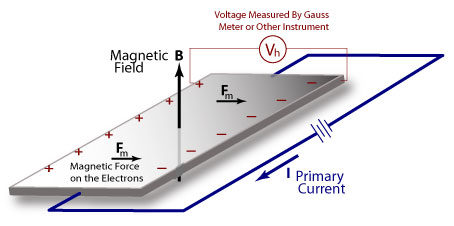
\includegraphics[width=0.6\linewidth]{./images/HallEffect.jpg}
        \caption{\label{HallEffect}Hall Effect}
    \end{figure}

    Hall sensors are mounted in a regular pattern around the motor as seen
    in figure \ref{BLDC:Sensor:Hall}
        \footnote{\url{https://homes.cs.washington.edu/~todorov/papers/SimpkinsACC10.pdf}}

    \begin{figure}
        \centering
        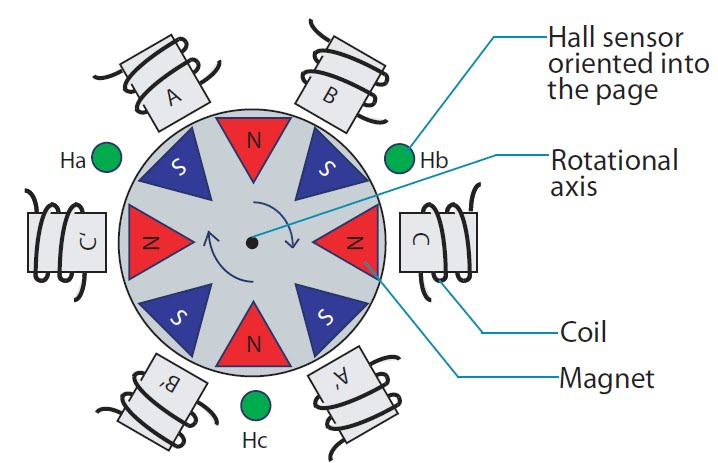
\includegraphics[width=0.6\linewidth]{./images/bldcHallSensors.jpeg}
        \caption{\label{BLDC:Sensor:Hall}Hall Sensors Layot for BLDC Motor}
    \end{figure}

    An important design consideration here, is to ensure there is no
    interference from the time-varying magnetic fields generated in the coils.
    Most setups follow the same layout as seen in figure \ref{BLDC:Sensor:Hall};
    this is either due to the fact that the sensor measures field strength in a
    narrow linear axis or that the reluctance of the air is far greater than the
    reluctance of the motor chassis, allowing the motor magnetic field to
    permeate to the sensor without interference from the coils.

\subsection{BLDC Motor Sensorless Control}
\footnote{\url{http://scholar.lib.vt.edu/theses/available/etd-09152003-171904/unrestricted/T.pdf}}
	\begin{enumerate}
	\item Sensorless control is bases on the back-emf produced by the motor
	\item There is a narrow range for which the back emf is sufficient to be detected
	\end{enumerate}
\end{document}
